\chapter{High Power RF Devices}
\label{chap:rf_power_devices}

\margintoc

\epigraph{There is all the difference in the world between knowing about and knowing how to do.}{James Evans, The History and Practice of Ancient Astronomy}


The purpose of RF engineering for plasma heating and current drive is to transmit several MW of RF power at frequencies from the MHz to GHz range and to deliver it into the plasma with the highest net efficiency as possible. The RF power is generated by one or few RF generators, then eventually combined and transported to the antennas. In order to optimize the global efficiency, it is desirable to have low loss, high electrical efficiency, low reflections, high reliability and actuators to adjust amplitude and phase. 

This chapter review the work done on high power RF devices at CEA/IRFM. The first section (\ref{sec:RF_fundamentals}) is a reminder of the essential elements of RF engineering and readers aware of the transmission line and electromagnetic networks can skip this section. 
ICRH and LHCD high power transmission line elements are detailed in section \ref{sec:RF_components} while the section \ref{sec:RF_antennas} is dedicated to the antenna designs. Since RF breakdowns are a recurrent problematic in high RF power applications, the section~\ref{sec:Multipactor} is fully dedicated to this topic, in particular to the multipactor phenomenon which occurs in vacuum environments.



% #####################################################
% #####################################################
% #####################################################
\section{RF Fundamentals}\label{sec:RF_fundamentals}

% #####################################################
% #####################################################
% #####################################################
\subsection{Uniform Transmission lines Properties}
\marginnote[*-2]{Part of this section are taken from the documentation of the open-source Python package \href{http://scikit-rf.org/}{scikit-rf} which is developed by the author and used in RF circuit models, for example in \citeauthyear{hillairet2015-2} or in \citeauthyear{hillairet2019-1}.}

Once RF waves have been generated, it must be transmitted to the antennas, using suitable transmission line depending on the RF frequency and power level. The main results and properties of uniform transmission lines are reviewed in this section. The results given here are well-known and can be found in numerous textbooks such as \sidecite{Harrington2001, marcuvitz1951, Thourel1988, Collin1990, gonzalez1997, pozar2012, Orfanidis, steer2019-3} to give a personal selection.

A transmission line is defined as \textit{uniform} if its dimensions and electrical properties are identical for all planes transverse to the direction of propagation. The results listed in this section are used in the following sections of this chapter for the design and the analysis of high power RF components.

% #####################################################
\subsubsection{Voltage and Current}

\begin{figure}
	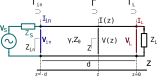
\includegraphics[width=1.0\textwidth]{figures/chap3/transmission_line_properties_vi}
	\caption{A transmission line terminated in a load impedance $Z_L$.}
	\label{fig:transmissionlinepropertiesvi}
\end{figure}

Let a lossy transmission line of propagation constant $\gamma=\alpha+j\beta$ (in $\si{m^{-1}}$) and characteristic impedance $Z_0$ (in $\si{\Omega}$), terminated by an arbitrary load $Z_L$. The line length is The source is parametrized by the distance $z$, where the source is located at distance $z=-d$ from the load ($z=0$) as illustrated in Figure~\ref{fig:transmissionlinepropertiesvi}. Attenuation constant $\alpha$ has the units of Nepers per meter $\si{Np/m}$ and the phase constant $\beta$ has the units radians per meter $\si{rad/m}$\footnote{$1\,\si{Np/m}$ equals to $8.6859 \, \si{dB/m}$. To convert from \si{dB} to \si{Np} multiply by $0.1151$. Thus $\alpha = x \, \si{dB/m} = x \times 0.1151 \, \si{Np/m}$.}. Let $V=V(z)$ and $I=I(z)$ the total voltage and current on the line, which can be written as a sum of a forward and reflected waves:
\marginnote{$\Vfwd$ and $\Vrefl$ ($\Ifwd$ and $\Irefl$) are defined here as peak voltages (currents). For sine wave, RMS voltage is $V_{\mathrm{RMS}}=V_{\mathrm{peak}}/\sqrt{2}$.}
\begin{subequations}
\begin{align}
	V(z) = \Vfwd(z) + \Vrefl(z) =& \Vfwd e^{-\gamma z} + \Vrefl e^{+\gamma z} \\
	I(z) = \Ifwd(z) + \Irefl(z) =& \frac{\Vfwd}{Z_0} e^{-\gamma z} - \frac{\Vrefl}{Z_0} e^{+\gamma z}
\end{align}
	\label{eq:voltage_current_lossy_line}
\end{subequations}
where the $e^{-\gamma z}$ term represents wave propagation in the $+z$ direction (and $e^{+\gamma z}$ in the $-z$ direction). The terms $\Vfwd$, $\Vrefl$ ($\Ifwd$, $\Irefl$) represent the forward and reflected voltage (current) waves at $z=0$.  
The \textit{characteristic impedance} $Z_0$ associated to a uniform transmission line (or any continuous media supporting the propagation of electromagnetic waves) is defined as the ratio of the forward voltage and current when the transmission line is infinite, i.e.  $Z_0=\Vfwd/\Ifwd(=-\Vrefl/\Irefl)$. It characterizes the property of the line to oppose a change in voltage for a change of current or vice-versa. When $Z_L=Z_0$, the load is said to be \textit{matched} to the line and there is no reflected wave $\Vrefl=0$.

\begin{marginfigure}[-2cm]
	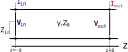
\includegraphics[width=1\linewidth]{figures/chap3/transmission_line_transfer}
	\caption{Propagation of current and voltage in a piece of uniform transmission line.}
	\label{fig:transmission_line_transfer}
\end{marginfigure}

The voltage and current at the input ($z=-d$) of a piece of uniform transmission line can be related to the voltage and current at its output (chosen at $z=0$) using the transfer matrix \sidecite{vittoria1998}:
\begin{equation}
\left( 
\begin{array}{c}
	V_{\mathrm{in}} \\
	I_{\mathrm{in}}
\end{array}
\right)
=
\left( 
\begin{array}{cc}
\cosh  \left(\gamma d\right) & Z_0 \sinh \left(\gamma d \right) \\ 
\frac{1}{Z_0}\sinh \left( \gamma d\right) & \cosh\left(\gamma d\right) 
\end{array} 
\right)
\left( 
\begin{array}{c}
	V_{\mathrm{out}} \\
	I_{\mathrm{out}}
\end{array}
\right)
	\label{eq:voltage_current_transfer_matrix}
\end{equation}




% #####################################################
\subsubsection{Reflection Coefficient}
The ratio of the reflected to forward voltage (or current) at a distance $z$ defines the \textit{reflection coefficient} $\Gamma$:
\marginnote{\textit{Return loss} RL is the negative of the magnitude of the reflection coefficient in \si{dB}. Since power is proportional to the square of the voltage, return loss is given by $$\mathrm{RL} = -20 \log_{10} |\Gamma|$$
The \textit{transmission coefficient} can be also defined as $$T=1+\Gamma$$
 sometime expressed as the \textit{insertion loss} IL in \si{dB}:
 $$\mathrm{IL}=-20 \log |T|$$}
\begin{equation}
\Gamma(z) = \frac{\Vrefl(z)}{\Vfwd(z)} =  \frac{\Irefl(z)}{\Ifwd(z)} = \Gamma_L e^{2\gamma z}
\label{eq:Gamma_at_z}
\end{equation}
where $\Gamma_L$ is the reflection coefficient of the load ($z=0$), given by:
\begin{equation}
	\Gamma_L = \frac{Z_L - Z_0}{Z_L + Z_0}
	\label{eq:Gamma_L}
\end{equation}
Note that the reflection coefficient at the input of the line $\Gamma_{\mathrm{in}}$ (Figure~\ref{fig:coaxial_line_fields}) is given for $z=-d$:
$$
\Gamma_{\mathrm{in}}=\Gamma(z=-d)=\Gamma_L e^{-2\gamma d}
$$

In fusion application, the load is unfortunately rarely matched to the transmission line or the source impedances, so it is convenient to re-express voltage and current equations (\ref{eq:voltage_current_lossy_line}) as a function of $\Gamma_L$ (\ref{eq:Gamma_L}) or $\Gamma(z)$ (\ref{eq:Gamma_at_z}):
\begin{subequations}
	\begin{align}
		V(z) =& \Vfwd \left( e^{-\gamma z} + \Gamma_L e^{+\gamma z} \right) 
			= \Vfwd \left[ 1 + \Gamma(z) \right]  e^{-\gamma z} \\
		I(z) =& \frac{\Vfwd}{Z_0} \left( e^{-\gamma z} - \Gamma_L e^{+\gamma z} \right)
			= \frac{\Vfwd}{Z_0} \left[ 1 - \Gamma_L(z)  \right]e^{-\gamma z}
	\end{align}
	\label{eq:voltage_current_lossy_line_gamma}
\end{subequations} 

The \textit{standing wave ratio} or SWR is defined as:
\marginnote[*-1]{With the inverse expression
	$$ 	|\Gamma| = \frac{\SWR - 1}{\SWR + 1} $$}
\begin{equation}
	\SWR(z) = \frac{1 + |\Gamma(z)|}{1 - |\Gamma(z)|}
	\label{eq:SWR}
\end{equation}
The SWR can be equivalently defined as the ratio of maximum (forward and backward waves are in phase) to minimum (forward and reflected waves are out of phase) voltage magnitudes: 
\begin{equation}
\SWR(z) = \frac{|V_\mathrm{max}(z)|}{|V_\mathrm{min}(z)|} = \frac{|\Vfwd|e^{-\alpha z} + |\Vrefl|e^{+\alpha z}}{|\Vfwd|e^{-\alpha z} - |\Vrefl|e^{+\alpha z}}
\label{eq:SWR_max_to_min_voltages}
\end{equation}
Note that the SWR becomes constant for lossless lines. 


Finally, some special cases are reminded for convenience in the Table~\ref{tab:special_case_loaded_line}.

\begin{table}[h]
	\begin{center}
\begin{tabular}{|c|c|c|}
	\hline 
	Case & $\Gamma$ & $\SWR$ \\ 
	\hline 
	Matched: $Z_L = Z_0$ & 0 & 1 \\ 
	\hline 
	Short: $Z_L=0$ & -1 & $\infty$ \\ 
	\hline 
	Open: $Z_L = \infty$ & 1 & $\infty$ \\
	\hline
\end{tabular}
	\end{center}
\caption{Special cases of a uniform loaded transmission line.}
\label{tab:special_case_loaded_line} 
\end{table}


% #####################################################
\subsubsection{Line Impedance}
The impedance seen toward the load at a point of the line, that is the ratio between total voltage and current at this point, is at a distance $z=-\ell$ from the load:
\begin{subequations}
	\begin{align}
Z(z=-\ell) 
	=& Z_0 \frac{Z_L + Z_0 \tanh( \gamma \ell)}{Z_0 + Z_L \tanh(\gamma \ell)} \\
	=& Z_0 \frac{1 + \Gamma(-\ell) }{1 - \Gamma(-\ell) }
	\end{align}
\end{subequations}
As noted aboved with respect to Figure~\ref{fig:coaxial_line_fields}, we have in particular $Z_{\mathrm{in}}=Z(z=-d)$ and $Z(z=0)=Z_L$.

% #####################################################
\subsubsection{Power and losses}\label{sec:power_and_losses}
The time average power flowing along the transmission line is the difference between the forward and the reflected powers:
\begin{equation}
P (z) = \frac{1}{2} \Re\left[V(z) I^*(z)\right] 
\label{eq:power_time_average_general}
\end{equation}

\marginnote{An example in the \href{https://scikit-rf.readthedocs.io}{scikit-rf package documentation} is dedicated to the evolution of the power, voltage, current and SWR in lossy line. See \cite[§2.7]{pozar2012}, \cite[§2.5.5]{steer2019}, \cite[§3-4c]{Rizzi1988} for discussions of power in lossy terminated line.}

For a lossy transmission line ($\alpha>0$), not all the power entering the transmission line will be delivered to the load as some power will be lost on the line due to attenuation. The time average power at any point of the transmission line (\ref{eq:power_time_average_general}) can be shown to be \sidecite[+1cm]{vernon1969, marks1992}:
\begin{subequations}
\begin{align} 
	P(z) =& P_\mathrm{f} - P_\mathrm{r} - P_\mathrm{c} \\
	P_\mathrm{f} =& \Re(Z_0) \frac{|V_\mathrm{f}|^2}{2 |Z_0|^2} e^{-2\alpha z} \\
	P_\mathrm{r} =& \Re(Z_0) \frac{|V_\mathrm{r}|^2}{2 |Z_0|^2} e^{+2\alpha z} = P_\mathrm{f} |\Gamma_L|^2 e^{+4\alpha z} \\
	P_\mathrm{c} =& \Im(Z_0) \Im\left[\frac{\Vrefl\Vfwd^*}{|Z_0|^2} e^{-2j\beta z} \right]
\end{align}
\end{subequations}
where $P_\mathrm{f}$ and $P_\mathrm{r}$ are the forward and reflected power respectively. In lossy lines, the net power flow $P(z)$ is not in general the difference of the forward and reflected power but carries an additional term $P_\mathrm{c}$. $P_\mathrm{c}$ can be either positive or negative along the line and is null for all $z$ only for a distortion-less line ($\Im(Z_0)=0$). In a word, the superposition of power does not apply in lossy uniform transmission lines (but superposition of voltages and currents does).

Keeping the notation used in Figure~\ref{fig:transmissionlinepropertiesvi} and using equations (\ref{eq:voltage_current_lossy_line_gamma}), the power delivered to the load (at position $z=0$) and at the input of the line (at position $z=-d$) are:
\begin{subequations}
	\begin{align}
		P_{\mathrm{L}} = P(z=0) =& \Re(Z_0) \frac{\left| \Vfwd \right|^2}{2 |Z_0|^2} \left(1 - |\Gamma_L|^2 \right) \\
		P_{\mathrm{in}} = P(z=-d) =& \Re(Z_0) \frac{\left| \Vfwd \right|^2}{2 |Z_0|^2} \left(1 - |\Gamma_L|^2 e^{-4\alpha d}  \right) e^{2\alpha d}
	\end{align}
\end{subequations}
hence the power lost in the line is:
\marginnote{The total loss $\mathrm{ML}$ in a line in \si{dB} can also be stated as:
$$
 \mathrm{TL}=10\log_{10} \left( \frac{A^2 - |\Gamma_L|^2}{A(1 - |\Gamma_L|^2)} \right)
$$
where $A=10^{\mathrm{ML}/10}$ and $\mathrm{ML}$ the matched line loss. The additional loss caused by the standing waves is the difference between the  $\mathrm{TL}$ and  $\mathrm{ML}$.
}
\begin{equation}
P_{\mathrm{loss}} = P_{\mathrm{in}} - P_{\mathrm{L}} 
= \Re(Z_0)  \frac{\left| \Vfwd \right|^2}{2 |Z_0|^2} 
\left[ 
\left(e^{2\alpha d} - 1\right) + |\Gamma_L|^2 \left( 1 - e^{-2\alpha d} \right)
\right]
\label{eq:power_loss_lossy_transmission_line}
\end{equation}
where the first and second terms in (\ref{eq:power_loss_lossy_transmission_line}) account for the power loss of the forward and reflected waves respectively.
	


For lossless transmission line and real characteristic impedance, the time average power flow along the transmission line is constant and (\ref{eq:power_time_average_general}) simplifies to:
\begin{equation}
P = P_\mathrm{f} - P_\mathrm{r} = P_\mathrm{f} \left(1 - |\Gamma_L|^2\right)
\label{eq:power_loss_lossless_transmission_line}
\end{equation}
This power can also be related to the maximum voltages or currents and $\SWR$ from Eq.(\ref{eq:SWR_max_to_min_voltages}):
\begin{equation}
P = P_\mathrm{f} - P_\mathrm{r} = \frac{1}{2 Z_0} \frac{	|V_{\mathrm{max}}|^2}{\SWR} = \frac{Z_0}{2} \frac{|I_{\mathrm{max}}|^2}{\SWR}
\label{eq:power_loss_lossless_transmission_line_maxvoltage_maxcurrent}
\end{equation}
where $|V_{\mathrm{max}}| = \max_z |V(z)| = |\Vfwd| + |\Vrefl|$ and similarly for $|I_\mathrm{max}|$. Combining the above two expressions leads to convenient formulas for heat flux and breakdown estimations, which relates the maximum (peak) voltage or current to the forward power $P_\mathrm{f}$ and reflection coefficient $|\Gamma_L|$:
\begin{subequations}
	\begin{align}
		|V_\mathrm{max}| =& \sqrt{2 Z_0 P_\mathrm{f} } \left(1 + |\Gamma_L| \right) \\
		|I_\mathrm{max}| =& \sqrt{\frac{2 P_\mathrm{f}}{Z_0} } \left(1 + |\Gamma_L| \right)
	\end{align}
	\label{eq:max_current_function_forward_power_gammaL}
\end{subequations}

The power lost in the transmission line is converted into heat in the metallic conductors and dielectric elements due to Ohmic and dielectric losses respectively. For high power applications such as RF heating and current drive, this heat must be evacuated to sustain CW operation. Before expressing loss formulas for the main two kinds of transmission lines used for ICRH and LHCD, we recall here for future references that the power loss in a good conductor can be calculated as:
\begin{equation}
P_\ell = \frac{R_s}{2} \int_S |J_s|^2 \diff S = \frac{R_s}{2} \int_S |H_t|^2 \diff S 
\label{eq:power_loss_conductor}
\end{equation}
where the integral is performed over the conductor surface(s), $J_s$ and $H_t$ the surface current and the tengential magnetic field respectively\cite[§1.7]{pozar2012}. 

definition of the \textit{skin depth} $\delta_s$ (in $[\si{m}]$) as:
\begin{equation}
\delta_s 
	=
	\sqrt{\frac{2}{\omega \mu \sigma}}
	\label{eq:skin_depth}
\end{equation}
and the \textit{sheet resistance} $R_s$ (in $[\si{\Omega}]$) as:
\begin{equation}
R_s 
	= 
	\frac{1}{\delta_s \sigma}
	=
	\sqrt{\frac{\omega\mu}{2\sigma}}
	=
	\sqrt{\pi f \rho \mu }
	\label{eq:sheet_resistance}
\end{equation}
with $\sigma=1/\rho$ the metal conductivity (in $[\si{S/m}]$) and $\sigma$ the metal resistivity (in $[\si{\Omega m}]$). 

% #####################################################
% #####################################################
\subsection{Matching Systems}
In high power RF systems for fusion applications, the load is ultimately the plasma facing the antennas. As seen in Section~\ref{sec:icrh} and Section~\ref{sec:lhcd}, the plasma loading impedance is generally small compared to antenna and transmission line. Hence, a significant amount of RF power will be reflected toward the generators. It is essential to protect high power RF sources (tetrodes, klystrons) from reflected power (output mismatch). Reflected power perturbs the source impedance, the output amplitude and phase and creates higher dissipation losses\sidecite[-1cm]{pompon2012}. It can also lead to the failure of RF windows \sidecite[-+0.5cm]{ikeda1989} or even damage the tube itself\sidecite{gold1997,carter2005,benford2007}. 

Unfortunately, the plasma characteristics depend on the machine setup but also on its history, hence its RF load properties are relatively little known in advance. In addition, plasma intrinsic instabilities, such as Edge Localized Modes (ELMs), can also induce strong and fast load variations in front of the antenna, which may affect strongly the generator performances for the aforementioned reasons\sidecite{braun1995, beaumont1996} or generate breakdown in antennas and transmission lines due to peak voltage increases \sidecite{bobkov2003-1, goniche2012-2}. 

\begin{marginfigure}[*+5]
	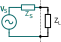
\includegraphics[width=0.8\linewidth]{figures/chap3/transmission_line_matching}
	\caption{Matching a load impedance $Z_L$ to a source having an internal impedance $Z_S$.}
	\label{fig:transmission_matching}
\end{marginfigure}

Let us consider the simplified network illustrated in Fig.\ref{fig:transmission_matching}. Classical results of RF engineering state that\cite{Rizzi1988, pozar2012}:
\begin{itemize}
	\item Conjugate Matching: maximum available power goes into the load if $Z_L=Z_S^*$
	\item Impedance Matching: minimum reflection ($\Gamma_L=0, \SWR=1$) is obtained for $Z_L=Z_S$
\end{itemize} 
As in typical plasma application the load impedance $Z_L$ is complex-valued, achieving both objectives at the same time is not possible. For this reason, a set of matching networks must be inserted between the source and the load as illustrated in Fig.~\ref{fig:transmission_matching_system}. Ideally, such a matching system should meet the following objectives (sometimes interrelated):
\begin{itemize}
	\item maximize the power transfer to the antenna 
	\item minimize the power reflected to the generator (protection and efficiency)
	\item minimize the power lost in the transmission line (net efficiency)
	\item insure the good control of the antenna amplitude/phase
\end{itemize}

If the generator is not equipped with internal matching network, it is a good engineering practice to place a matching network as close as possible from its output. Similarly, placing a matching network as close as possible from the load reduce the standing waves and thus the peak current (dissipation problems) and the peak voltage (corona and breakdown problems) in the transmission line between the source and the load \cite[§4]{Rizzi1988}.

\begin{figure}
	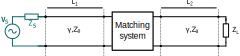
\includegraphics[width=1\linewidth]{figures/chap3/transmission_line_matching_system}
	\caption{A matching system is inserted between the source and the load impedance.}
	\label{fig:transmission_matching_system}
\end{figure}

Matching is frequency dependant since it deals with the adjustment of reactances. The perfect impedance match can occur only at one frequency but high power sources are usually very narrowband. If the source frequency can be tuned, which is the case of ICRH generators, matching networks are designed to be tunable. Such system use stub (shunt coaxial section that ends in a movable short) and line stretchers (transmission line section that can vary its electrical distance). In theory, a one-quarter-wavelength stub in conjunction with a half-wavelength stretcher can match any impedance to the generator\sidecite{england1989}. However, the actuators of these systems rely on motors (capacitors) or hydraulic systems (tuning stub, line stretchers), so their response time is of the order to 100 milliseconds or higher, which is much slower than most uncontrolled plasma variations. For this reason, fusion RF antenna are designed to be intrinsically relatively load-tolerant, using specific feeding line or antenna design. 


% #####################################################
% #####################################################
\subsection{Scattering Parameters}
Voltage  $V(z)$ and current $I(z)$ as defined in Eq.(\ref{eq:voltage_current_lossy_line}) in the previous section are the "real" waves in the sense that they are linked directly to Maxwell’s equations and can be measured. For example, reflection coefficients $\Gamma(z)$ can be measured from the peaks and valleys of the electric fields of the standing wave created by the beating of forward and reflected voltages and currents in a slotted-line experiment \sidecite{marks1992, williams2013}. 

A RF \textit{network} such as the one illustrated in Fig.~\ref{fig:microwave_network}, is a system for which a closed surface separating the network from the rest of the world can be found such that it has zero current on this surface ($\hat{\mathbf{n}} \times \Ebf=0$) except over one or more input/output \textit{port} cross-section \cite[§8.3]{Harrington2001}. The electrical behaviour of linear electrical networks is often handled using impedances or admittances parameters, relating voltages to currents at each port (or reference planes). Direct measurements of these impedances or admittances of a RF network requires that the ports be terminated in either short or open circuits. However, as lead inductance and capacitance make short and open circuits difficult to obtain at RF frequencies, such terminations are often hard to realize correctly. Since power transfer is often a crucial characteristic of RF network designs, \textit{scattering parameters} (or S-parameters) are often preferred by microwave engineers since they relate the power flow of forward and reflected voltage waves at each port. Finally, scattering parameters are also well suited for describing transistors and other active devices, since short and open  terminations could result in undesired behavior, including oscillation or destruction\sidecite{steer2019-1}.

\begin{marginfigure}[*-15]
	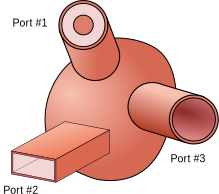
\includegraphics[width=1\linewidth]{figures/chap3/microwave_network}
	\caption{A 3 ports RF Network.}
	\label{fig:microwave_network}
\end{marginfigure}

Scattering parameters can be defined in several ways \sidecite{dobrowolski2010}, which has been discussed extensively in the literature since the 60's \cite{carlin1956, kurokawa1965, woods1972, marks1992, williams2013, amakawa2016}. Indeed, there is some arbitrariness to define some forward and reflected waves ($a, b$) such that ($|a|^2, |b|^2$) represent the time-averaged power carried by the forward and reflected voltage waves ($\Vfwd, \Vrefl$) (or current waves, or both). However, as seen in section \ref{sec:power_and_losses}, the power superposition principle does not hold for lossy lines and complex characteristic impedances (but superposition of voltages and currents does), so this mapping cannot be done in general. The various definitions of scattering parameters differ on how they handle complex impedances and eventually additional modes other than TEM, but all of these definitions give the same results for real-valued characteristic impedances and lossless lines\footnote{Because most of time lossless lines are assumed, this is probably the reason why most textbooks assume that the characteristic impedance is real in their presentation of scattering parameters. While complex-referenced S-parameters may be seen as a matter of purely academic concern with little practical use, it is not and it has also implications in electromagnetic simulators that are often silent on how they implement such situations.}. To deal with lossy lines and complex characteristic impedances, few methodologies exist but two are nowadays mostly adopted: \textit{power-wave} and \textit{pseudo-wave}  definitions. 

The \textit{power-waves} concept has been introduced in \sidecite{kurokawa1965}, where the forward $a$ and reflected $b$ power-waves are defined as:
\begin{subequations}
\begin{align}
	a =& \frac{V_i + Z_{R,i} I_i}{2\sqrt{|\Re(Z_{R,i})|}} \\
	b =& \frac{V_i - Z_{R,i}^* I_i}{2\sqrt{|\Re(Z_{R,i})|}}
\end{align}
\label{eq:power-waves_definition}
\end{subequations}
where $V_i$ and $I_i$ are the total voltage and current flowing into the $i$th port of the network. $Z_{i}$ is the $i$th port reference impedance. The choice of the reference impedance is free; a common practice is to set its value to the impedance of a load or a generator, enabling power waves to be used in matching problems. With power-waves, the power flowing at the port interface is:
\begin{equation}
	p_{\mathrm{pw}} = \frac{1}{2} \left( |a|^2 - |b|^2 \right)
\end{equation}

As seen in the previous section, impedance match and maximum power transfer are in general not coincident. For the latter condition, a conjugate match is required, i.e. when $Z_0 = Z_L^*$ using the notation of Fig.~\ref{fig:transmissionlinepropertiesvi}. Power-waves are defined in such a way that a conjugate match produces no reflection, and also in such a way that the incident wave carries the available power of the source and the reflected wave the total reflected power from the load\sidecite{woods1972}. Thus, the power-wave reflection coefficient is defined by:
\marginnote{To be compared with Eq.(\ref{eq:Gamma_L}).}
\begin{equation}
	\Gamma_{\mathrm{pw}} = \frac{Z_0 - Z_L^*}{Z_0 + Z_L}
\end{equation}

This definition introduces "wave" variables that can no longer be interpreted as incoming and outgoing waves from ports. However, they can be interpreted in terms of power flow at a junction, which explains its wide adoption by the RF community. Most RF circuit solvers (such as Keysight ADS, ANSYS Circuit) use the \textit{power-waves} definition introduced. \marginnote[*-4]{Because of its wide adoption, \href{http://scikit-rf.org/}{scikit-rf} also uses the power-waves definition by default (mostly in order to replicate results from commercial solvers) but allows the use of pseudo-wave definition as well.} 

However, the power-wave definition has some caveats one must be aware of. In particular, power-waves definition may not give physical results in case of complex characteristic impedance\footnote{A simple illustration of the problem is to consider a transmission line of complex characteristic impedance $Z_0$ loaded with a an impedance $Z_L=Z_0^*$. Voltage and current waves as defined at the beginning of this section will lead to a non zero reflection coefficient $\Gamma_L$ while power-waves-based tools will give a zero reflection coefficient $\Gamma_\mathrm{pw,L}$\cite{amakawa2016}.} and are not always continuous at the interface between circuits unless reference impedance is real, so cannot be cascaded in all cases{marks1992, williams2013}. In the real world, all transmission lines are lossy (at least to a small degree) and this contradiction has been identified shortly after Kurokawa seminal paper\cite{amakawa2016} but somewhat forgotten after. For this reason, \citeauthyear{marks1992} introduced the \textit{pseudo-waves} definition of S-parameters\footnote{where a phase factor used in \cite{marks1992} has been omitted here for simplification.}:\marginnote{Again, the pseudo-wave definition equals the travelling-wave definition when $\Zref$ is real-valued. This paragraph aims only to highlight the fact that great care should be taken when dealing with S-parameters with lossy transmission lines with electromagnetic solvers, in particular closed-source ones.}
\begin{subequations}
	\begin{align}
		a_i =& \frac{\sqrt{\Re(Z_{R,i})}}{|Z_{R,i}|} \Vfwd_i 
		= \frac{\sqrt{\Re(Z_{R,i})}}{|Z_{R,i}|} \frac{V_i + Z_{R,i} I_i}{2} \\
		b_i =& \frac{\sqrt{\Re(Z_{R,i})}}{|Z_{R,i}|} \Vrefl_i 
= \frac{\sqrt{\Re(Z_{R,i})}}{|Z_{R,i}|} \frac{V_i - Z_{R,i} I_i}{2}		
	\end{align}
\end{subequations}
where $Z_{R,i}$ is an arbitrary value which can be different from the characteristic impedance $Z_0$ of the physical transmission line at the $i$th port. $a$ and $b$ are not longer directly related to voltage and curent travelling wave and only when $Z_{R}$ equals to $Z_0$ do $a$ and $b$ correspond to actual travelling wave amplitude (normalized to unit of $\sqrt{\si{W}}$). The power $p$ transmitted by a pseudo-wave at the port interface is:
\begin{equation}
p = \frac{1}{2} \left(|a|^2 - |b|^2 - 2\Im(a^* b) \frac{\Im(\Zref)}{\Re(\Zref)} \right)
\end{equation}

For a N-port network, with both definitions, the forward and reflected waves are related by:
\begin{equation}
	\bbf = \Sbb \abf
\end{equation}
where the $\abf$ and $\bbf$ array are constituted of the $a_i$ and $b_i$ elements. Properties of S-matrices are discussed in \sidecite{gonzalez1997, dobrowolski2010} to name of few and are not covered here.




% #####################################################
% #####################################################
\subsection{Coaxial Lines}\label{sec:coaxial_lines}
% #####################################################
\subsubsection{Coaxial Lines Main Properties}
A coaxial line is made of two cylindrical conductors, the internal of radius $a$ and the external of radius $b$, encapsulated one inside the other as illustrated in Figure~\ref{fig:coaxial_line_geometry}. The space between both conductors is filled with a dielectric. In high power application, conductors are made of rigid metallic cylinder (aluminium or stainless steel) eventually copper or silver coated to reduce RF losses. The dielectric is simply (dry) air, pressurized nitrogen or vacuum to reduce dielectric breakdown. 

% #####################################################
\subsubsection{Electric and Magnetic Fields}
The fundamental mode in a coxial line is a TEM mode as both electric and magnetic field are transverse to the propagation direction. This mode has no cut-off and therefore coaxial can be used down to DC.

\begin{marginfigure}[*-10]
	
\includegraphics[width=1\linewidth]{figures/chap3/coaxial}
	\caption{Coaxial Line Geometry}
	\label{fig:coaxial_line_geometry}
\end{marginfigure}

The electric and magnetic field inside the coaxial are illustrated in Figure~\ref{fig:coaxial_line_fields} and given by:
\begin{subequations}
	\begin{align}
		\Ebf(r) =& \frac{V}{r \ln \left(b/a \right)} \hat\ebf_r \label{eq:coaxial_electric_field}\\
		\Hbf(r) =& \frac{I}{2\pi r} \hat\ebf_\phi \label{eq:coaxial_magnetic_field}
	\end{align}
	
\end{subequations}
where $V=V_0 e^{\mp\gamma z}$ is the voltage between the conductors and $I=I_0 e^{\mp\gamma z}$ is the current in each conductor, for $a\leqslant r \leqslant b$. 

\begin{marginfigure}[*-8]
	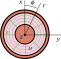
\includegraphics[width=.8\linewidth]{figures/chap3/coaxial_fields}
	\caption{TEM mode for a coaxial line}
	\label{fig:coaxial_line_fields}
\end{marginfigure}	

% #####################################################
\subsubsection{Characteristic Impedance}. 
The characteristic impedance $Z_0$ in $[\si{\Omega}]$ of a coaxial line is:
\begin{equation}
Z_0 = 
	\frac{1}{2\pi} \sqrt{\frac{\mu_0 \mu_r}{\varepsilon_{0} \varepsilon_{r}}} \ln\left( \frac{b}{a} \right)
	=
	60 \sqrt{\frac{\mu_r}{\varepsilon_{r}}} \ln\left( \frac{b}{a} \right) 
\end{equation}
\marginnote[-1cm]{Or also, $Z_0\approx 138 \sqrt{\frac{\mu_r}{\varepsilon_{r}}} \log_{10}\left( \frac{b}{a} \right)$}
with $\varepsilon_{r}$ the relative permittivity and $\mu_r$ the relative permeability of the filling dielectric. 

% #####################################################
\subsubsection{Power and Losses}
From Eq.(\ref{eq:coaxial_electric_field}), the maximum electric field is located on the inner conductor ($r=a$). The maximum voltage before breakdown $V_{\mathrm{max,bd}}$ is:
\begin{equation}
	V_{\mathrm{max,bd}} = a\ln\left(b/a\right) E_d
\end{equation}
where $E_d$ is the \textit{dielectric field strength} of the medium. For dry-air, this value is given as $3$~\si{MV/m} for dry air\cite[b§3.11]{pozar2012}.\marginnote{The field strength is vacuum is in theory much higher, however as detailed in Section~\ref{sec:Multipactor}, electrical breakdown in vacuum can occur because of other mechanisms.}. In a lossless coaxial line, the associated maximum power before breakdown $P_\mathrm{max,bd}$ is from Eq.(\ref{eq:power_loss_lossless_transmission_line})
\begin{equation}
	P_\mathrm{max,bd} =  \frac{V^2_{\mathrm{max,bd}} }{2 Z_0 \SWR}= \sqrt{\frac{\varepsilon_{r}}{\mu_r}} \frac{a^2 E_d^2}{120\,\SWR} \ln (b/a)
\end{equation}
This expression shows that the power capability can be increased by using a larger coaxial line for the same characteristic impedance or by increasing the $b/a$ ratio (higher characteristic impedance) and by reducing the $\SWR$.

The Ohmic heat flux $\Psi$ (in [$\si{W/m^2}$]) due to the flow of RF current on a conductor of diameter $\phi$ is given by:
\begin{equation}
\Psi(\phi,z) 
=
\frac{R_s}{2}
\frac{|I(z)|^2}{(\pi \phi)^2}
\label{eq:ohmic_heat_flux_coaxial}
\end{equation}
The previous expression can be used to calculate thermal behaviour of high power coaxial components (Fig.~\ref{fig:coaxial_losses}). The Ohmic power loss per unit length $P_\ell$ (in \si{W/m}) dissipated in a coaxial line is the sum of the inner and the outer conductors losses:
\begin{equation}
P_\ell (z)
=
\frac{1}{4 \pi}
\left(
\frac{R_{s,a}}{a} + \frac{R_{s,b}}{b}
\right)
|I(z)|^2
\end{equation}


\begin{figure}
	\centering
	\includegraphics[width=1.0\linewidth]{figures/chap3/coaxial_losses}
	\caption{Coaxial losses in a 2~meter 30~\si{\Omega} 9" coaxial line with $P_\mathrm{i}=500~\si{kW}$ and  $P_\mathrm{r}=300~\si{kW}$ at 100~\si{MHz}. Inner conductor is in copper while the outer conductor is in aluminium. Heat flux from Eq.(\ref{eq:ohmic_heat_flux_coaxial}) is benchmarked against full-wave ANSYS HFSS.}
	\label{fig:coaxial_losses}
\end{figure}

%Finally, the attenuation $\alpha=P_\ell(z=0)/(2P_0)$ in $[\si{Neper/m}]$ of a coaxial line is\cite[Ex.2.7]{pozar2012}:
%\begin{equation}
%\alpha 
%	=
%	\frac{1}{4\pi Z_0}
%	\left(
%		\frac{R_{s,a}}{a} + \frac{R_{s,b}}{b}
%	\right)
%	+
%	\frac{1}{2}\omega \varepsilon'' \eta
%\end{equation}
%where $R_{s,a}$ and $R_{s,b}$ are the sheet resistances given by eq.\ref{eq:sheet_resistance} for inner and outer conductors respectively and $\eta=\sqrt{\mu/\varepsilon'}$ is the intrinsic impedance of the dielectric material filling the coaxial line. 

% #####################################################
% #####################################################
\subsection{Rectangular Waveguides}\label{sec:rectangular_waveguide}
\subsubsection{Rectangular Waveguides Main Properties}
Electromagnetic wave can also propagate in hollow metallic structures filled with dielectric. The structure dimensions must be designed to the wavelength to transport. Waveguides can support different kinds of modes, the most conventiannol being TE (Transvere Electric) and TM (Transverse Magnetic) modes. 

\begin{marginfigure}[0cm]
	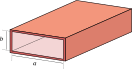
\includegraphics[width=1\linewidth]{figures/chap3/rectangular_waveguide}
	\caption{Rectangular Waveguide Geometry}
	\label{fig:rectangular_waveguide_geometry}
\end{marginfigure}

A hollow rectangular waveguide of width $a$ and height $b$ is illustrated in Figure \ref{fig:rectangular_waveguide_geometry}. Solving Maxwell’s equations for this geometry leads to multiple possible solutions, or \emph{modes}. In a rectangular waveguide, modes can be expressed as \emph{Transverse Electric} (TE) or \emph{Transverse Magnetic} (TM), depending of their respective polarization. Since the walls of a rectangular waveguide constrain the electromagnetic field boundary conditions along two dimensions, two integer indices $m$ and $n$ are used to describe a mode from another. Thus, modes in a rectangular waveguides can be $\TE_{mn}$ or $\TM_{mn}$\sidenote{With $m$ and $n$ integers greater or equal to 0 for $\TE$ modes and greater or equal to 1 for $\TM$ modes.}. These modes are eigenfunctions of the equation system and each mode is characterized by a wavenumber $\beta_{mn}$:
\begin{equation}
	\beta_{mn} = \sqrt{k^2_0 - k_{c,mn}^2 }
	\label{eq:rectwg_wavenumber}
\end{equation}
with $k_0=\omega\sqrt{\mu\varepsilon}=\sqrt{\mu_r \varepsilon_{r}}\omega/c$ and where $k_{c,mn}$ is the \textit{cut-off wavenumber}:
\marginnote{We recall here for convenience that the medium wavelength $\lambda$ is:
	$$
	\lambda = \frac{\lambda_0}{n} = \frac{v_\phi}{f}
	$$
	where $\lambda_0$ is the wavelength in vacuum, $v\phi$ is the phase velocity, $n=c/v_\phi=\sqrt{\mu_r \varepsilon_{r}}$ is the refractive index and $c=1/\sqrt{\mu_0 \varepsilon_{0}}$ the speed of light. We also define 
	$$
	\xi_0=\sqrt{\frac{\mu_0}{\varepsilon_{0}}}=120\pi=377\,\si{\Omega}
	$$ 
	as the vacuum characteristic impedance.
}
\begin{equation}
	k_{c,mn}
	=
	\sqrt{\left(\frac{m\pi}{a}\right)^{2}+\left(\frac{n\pi}{b}\right)^{2}}
	\label{eq:rectwg_cutoff_wavenumber}
\end{equation}

Each mode has an associated \textit{cut-off frequency} $f_{c,mn}$, below which a mode cannot propagate in the guide:
\begin{equation}
	f_{c,mn} = \frac{k_{c,mn}}{2\pi\sqrt{\mu \varepsilon}}
	\label{eq:rectwg_cutoff-frequency}
\end{equation}
The mode $mn$ can propagate in a rectangular waveguide only if the operating frequency is higher than the cut-off frequency of the mode, i.e. $f>f_{c,mn}$. The mode with the lowest cut-off frequency is called the \textit{fundamental} or \textit{dominant} mode. Because we have assumed that $a>b$, the lowest cut-off frequency occurs for the $\TE_{10}$ ($m=1,n=0$) mode\sidenote{There are no $\TE_{00}$ mode.}. 

For practical applications, the dimensions of the waveguides are generally chosen in order to have one and only one mode allowed propagating for a specified frequency band. Other modes can eventually be excited by waveguides discontinuities, but can’t propagate since they are evanescent ($k^2_0 < k_{c,mn}^2$ in Eq.(\ref{eq:rectwg_wavenumber})). Such modes are referred to \textit{high order modes}. For high power applications, a great care is given to waveguide inner walls, bends and connections, since reflected power and breakdowns may occur due to discontinuities in the conducting walls, such as the ones caused by flange misalignments \sidecite{harvey1955,brady1965,kerr2010}, bumps, holes, etc.

% #####################################################
\subsubsection{Electric and Magnetic Fields}
At a given frequency in a homogeneous-filled metallic hollow waveguide, the set of all possible TE and TM modes forms an orthogonal basis and a complete system\cite[§1.2]{marcuvitz1951},\cite[§5.2]{Collin1990},\cite[§8.2]{Harrington2001}. In practice, this sum is over all propagating modes and truncated to few evanescent modes only if needed, which is the case for antenna-plasma coupling calculations (Cf. Section~\ref{sec:lhcd}). In order to match the geometry usually used for plasma-wave coupling theory, we assume here that the large side of the waveguide is aligned in the direction $y$ and the short side in the direction of $z$. The waveguide cross-section is supposed homogenous in the $x$ direction. The geometry of a rectangular waveguide is illustrated in Fig.\ref{fig:rectangular_waveguide_geometry_fields}. The transverse electromagnetic fields can be expressed the summation of these modes:

\begin{marginfigure}[0cm]
	\includegraphics[width=1\linewidth]{figures/chap3/rectangular_waveguide_fields}
	\caption{Rectangular Waveguide Geometry and $\TE_{10}$ mode pattern derived from Eq.(\ref{eq:rectwg_EHfields_TE10})}
	\label{fig:rectangular_waveguide_geometry_fields}
\end{marginfigure}

\begin{subequations}
	\begin{align}
\mathbf{E}_{t}(\mathbf{r}) = & \sum_{p,m,n} V_{pmn}(x)\mathbf{e}_{pmn} (y,z)
\label{eq:E_guides_somme_modes}\\
\mathbf{H}_{t}(\mathbf{r}) = & \sum_{p,m,n} I_{pmn}(x)\mathbf{h}_{pmn} (y,z)
\label{eq:H_guides_somme_modes}
	\end{align}
\label{eq:rectwg_transverse_fields_sum_modes}
\end{subequations}
with $V_{pmn}$ and $I_{pmn}$ the eigenvalues of a mode $p=\{\TE,\TM\}$ of indexes $(m,n)$ and $\gamma_{pmn}=j\beta_{pmn}$ its associated wavenumber. 

\begin{subequations}
	\begin{align}
V_{pmn}(x) = & A_{pmn}e^{-\gamma_{pmn}x} + B_{pmn}e^{+\gamma_{pmn}x}
\label{eq:valeur_propre_V}\\
I_{pmn}(x) = & \frac{1}{Z_{pmn}}\left(A_{pmn}e^{-\gamma_{pmn}x} - B_{pmn}e^{+\gamma_{pmn}x}\right)
\label{eq:valeur_propre_I}
	\end{align}
	 \label{eq:rectwg_modes_eigenvalues}
\end{subequations}
with $Z_{pmn}$ the mode characteristic impedance:
\begin{equation}
Z_{pmn} = 
\begin{cases}
\frac{j\omega\mu}{\gamma_{mn}} = \frac{j k_0 \xi_0}{\gamma_{mn}} & \mathrm{\, for\, \TE\, modes}\\
\frac{\gamma_{mn}}{j\omega\varepsilon}=\frac{\gamma_{mn} \xi_0}{j k_0} & \mathrm{\, for\,\TM\, modes}
\end{cases}
\end{equation}

The model eingenfunction for rectangular waveguides are\cite[§2.2]{marcuvitz1951},\cite[§8.1,§8.2]{Harrington2001},\cite[§5.4]{Collin1990},\cite[§3.3]{pozar2012},\cite[Appendix A]{Bers1981} for TE modes:
\begin{eqnarray}
\mathbf{e}_{mn}^{\TE}(y,z) & = & -\ebf_x \times \mathbf{h}_{mn}^{\TE} = \ebf_x \times \nabla_{t} \psi_{mn}\\
\mathbf{h}_{mn}^{\TE}(y,z) & = &  \ebf_x \times \mathbf{e}_{mn}^{\TE} = -\nabla_{t} \psi_{mn}
\end{eqnarray}
and mode TM modes:
\begin{eqnarray}
\mathbf{e}_{mn}^{\TM}(y,z) & = & -\nabla_{t}\phi_{mn}\\
\mathbf{h}_{mn}^{\TM}(y,z) & = & \ebf_x \times\mathbf{e}_{mn}^{\TM}= -\ebf_x \times\nabla_{t}\phi_{mn}
\end{eqnarray}
The longitudinal components are given by:
\begin{eqnarray}
E_{x}^{TM} & = & \sum_{m,n}\frac{k_{c,mn}^{2}}{j k_{0}}\xi_0 I_{m,n}(x)\phi_{mn}(y,z)\\
H_{x}^{TE} & = & \sum_{m,n}\frac{k_{c,mn}^{2}}{j k_{0}}\xi_0^{-1} V_{m,n}(x)\psi_{mn}(y,z)
\end{eqnarray}
$\psi$ and $\phi$ are the generator functions (\emph{transverses field pattern mode functions}). For a rectangular waveguide\cite[Table 8.1]{Harrington2001}\cite[§1.2 (6.c),§2.2]{marcuvitz1951}\cite[Appendix A, A13-14]{Bers1981}:
\begin{eqnarray}
\psi_{mn} & = & \frac{1}{\pi}\sqrt{\frac{\epsilon_{m}\epsilon_{n}}{m^{2}\frac{b}{a}+n^{2}\frac{a}{b}}}\cos\left(\frac{m\pi}{a}y\right)\cos\left(\frac{n\pi}{b}z\right)\label{eq:fonction_generatrice_TE}\\
\phi_{mn} & = & \frac{2}{\pi}\sqrt{\frac{1}{m^{2}\frac{b}{a}+n^{2}\frac{a}{b}}}\sin\left(\frac{m\pi}{a}y\right)\sin\left(\frac{n\pi}{b}z\right)\label{eq:fonction_generatrice_TM}
\end{eqnarray}
where $\epsilon_{k}=1$ if $k=0$ or $\epsilon_{k}=2$ otherwise.

Since these solutions form a orthogonal basis, the following integral over the waveguide cross-section $S$ gets\cite{marcuvitz1951,Collin1990}:

\begin{equation}
\left\langle \mathbf{f},\mathbf{g}\right\rangle 
=
\iint_{S}\mathbf{f}(y,z)\mathbf{\cdot g}(y,z)\, \diff y\, \diff z
\label{eq:rectwg_scalar_product}
\end{equation}
in particular:
\begin{subequations}\label{eq:relations_orthogonalite}
	\begin{eqnarray}
	\left\langle \mathbf{e}_{mn}^{\TE},\mathbf{e}_{m'n'}^{\TE}\right\rangle  & = & \delta_{m=m',n=n'}\\
	\left\langle \mathbf{e}_{mn}^{\TE},\mathbf{h}_{m'n'}^{\TE}\right\rangle  & = & \delta_{m=m',n=n'}\\
	\left\langle \mathbf{e}_{mn}^{\TE},\mathbf{e}_{m'n'}^{\TM}\right\rangle  & = & 0\\
	\left\langle \mathbf{e}_{mn}^{\TE},\mathbf{h}_{m'n'}^{\TM}\right\rangle  & = & 0
	\end{eqnarray}
\end{subequations}
where $\delta_{m=m',n=n'}=1$ if $m=m'$ and $n=n'$, $0$ otherwise.

For the fundamental mode $\TE_{10}$ (with $a>b$), one has in particular:
\begin{subequations}
	\begin{align}
\psi_{10}(y) &= 
	\frac{1}{\pi} \sqrt{\frac{2a}{b}} \cos\left(\frac{\pi}{a} y\right) 
	\\
\Ebf_t(x,y) =& 
	-  \sqrt{\frac{2}{ab}} \sin\left(\frac{\pi}{a} y\right)V_{10}(x) \hat\ebf_z 
	\\
\Hbf_t(x,y) =& 
	   \sqrt{\frac{2}{ab}} \sin\left(\frac{\pi}{a} y\right)I_{10}(x)\hat\ebf_y 
	\\
H_x(x,y) =& 
	\frac{k_{c,10}^2}{j \omega\mu} \frac{1}{\pi} \sqrt{\frac{2a}{b}} \cos\left(\frac{\pi}{a} y\right) V_{10}(x)
	\end{align}
	\label{eq:rectwg_EHfields_TE10}
\end{subequations}
\marginnote[-3cm]{We we have used $\omega\mu=k_0\xi_0=\beta_{mn}Z_{mn}$.}

% #####################################################
\subsubsection{Power and Losses}
The previous choice of normalization factors leads to simple time-average power flow along a rectangular waveguide:
\begin{equation}
P=\iint\frac{1}{2}\Re\left[\mathbf{E}_{t}\times\mathbf{H}_{t}^{*}\right]\cdot \hat \ebf_x \diff S
=
\sum_{l}\frac{1}{2Z_{l}}\left(\left|A_{l}\right|^{2}-\left|B_{l}\right|^{2}\right)
\label{eq:poynting}
\end{equation}
where the sum is over the propagating modes only. 

Since the $\TE_{10}$ mode is the fundamental mode and the most used to transfer the RF power, we will specify some quantities for $m=1,n=0$. Using Eqs.(\ref{eq:rectwg_EHfields_TE10}), the power flow down the guide for the $\TE_{10}$ is:
\begin{equation}
	P_{10} = \frac{1}{2} \Re \iint_S  \left(\Ebf \times \Hbf^* \right)\cdot \hat\ebf_x \diff y \diff z
	= \frac{1}{2} \Re\left[V_{10}(x) I^*_{10}(x) \right]
	\label{eq:rectwg_poynting_TE10_V10_I10}
\end{equation}
which reads from Eqs.(\ref{eq:rectwg_modes_eigenvalues}):
\begin{equation}
	P_{10} = \frac{1}{2Z_{10}}\left(\left|A_{10}\right|^{2}-\left|B_{10}\right|^{2}\right)
	\label{eq:rectwg_poynting_TE10_A10_B10} = P_\mathrm{i} -  P_\mathrm{r}
\end{equation}
where $P_\mathrm{i}$ (in [\si{W}]) is the forward power and $P_\mathrm{r}$ the reflected power. Coefficients $|A_{10}|$ and $|B_{10}|$ can then be related conveniently to the forward and reflected power:
\begin{subequations}
	\begin{align}
	|A_{10}| =& \sqrt{2Z_{10} P_\mathrm{i}} \\
	|B_{10}| =& \sqrt{2Z_{10} P_\mathrm{r}} =  R |A_{10}|
	\end{align}	
\end{subequations}	
where we have used the "voltage" reflection coefficient $R$ defined by $R^2=P_\mathrm{r}/P_\mathrm{i}$. Using all the previous definitions, the electromagnetic field in Eqs.(\ref{eq:rectwg_EHfields_TE10}) can be directly related to forward and reflected powers, giving peak values comparable to full-wave calculations and for breakdown analysis. A simple benchmark of these relations is given on Fig.\ref{fig:rectwg_benchmark_fields}.

The electric field for the $\TE_{10}$ mode is maximum at $x=a/2$ (in the middle of the waveguide). This peak electric field value for this mode is:
\begin{equation}
	\left| E_{y,\mathrm{max}} \right|
	=
	2 \sqrt{\frac{Z_{10} P_\mathrm{i}}{a b }} 
		\left( 
			1 + R
		\right)
\end{equation}

The maximum incident power before breakdown for a given reflection coefficient in a dielectric-filled rectangular waveguide is thus:
\begin{equation}
	P_{\mathrm{max,bd}}
	= 
	\frac{a b}{4 Z_{10}} \frac{E_d^2}{\left(1 + R\right)^2}
\end{equation}
with $E_d$ the electric strength of the medium. The previous expression shows that the maximum power is again obtained for a minimum reflection coefficient and increase with the waveguide dimensions. 

The Ohmic loss is not homogeneous in a rectangular waveguide. The Ohmic power loss density (in [$\si{W/m^2}$]) is, for the large ($\Psi_a$) and the small ($\Psi_b$) sides of the waveguide respectively:
\begin{subequations}
	\begin{align}
		\Psi_a(x,y)
		=& \frac{R_s}{2} \left(\left| H_x(x,y) \right|^2 + \left| H_y(x,y) \right|^2 \right)
\\
		\Psi_b(x)
		=& \frac{R_s}{2} \left| H_x(x,0) \right|^2 
	\end{align}
\end{subequations}

From symmetry, the currents on the top and bottom walls are identical, as are the currents on the small walls. So, the Ohmic power loss per unit length $P_\ell$ (in \si{W/m}) for a waveguide is then: 
\begin{equation}
P_\ell (z)
= 
2\int_0^a  \Psi_a(x,z) \diff x 
+ 
2\int_0^b  \Psi_b(z) \diff y 
\end{equation}
which reads:
\begin{equation}
P_\ell (z)
= 
R_s \left[
	\frac{1}{b} \left| I_{10} \right|^2 
	+ 
	\left(
		2a + \frac{a^2}{b}
	\right)
	\frac{k_{c,10}^2}{(\omega\mu\pi)^2} 
	\left| V_{10} \right|^2 
\right]
\end{equation}

\begin{figure}
	\centering
	\includegraphics[width=1.0\linewidth]{figures/chap3/rectangular_waveguide_fields_losses}
	\caption{$E$ and $H$ fields and RF losses in a 400~\si{mm} WR284 waveguide ($72.13 \times 34.04$~\si{mm}) with $P_\mathrm{i}=500~\si{kW}$ and  $P_\mathrm{r}=100~\si{kW}$ at 3.7~\si{GHz}. Conductor are in copper. Results are  benchmarked against full-wave ANSYS HFSS.}
	\label{fig:rectwg_benchmark_fields}
\end{figure}














% #####################################################
% #####################################################
\section{ICRH Antennas}\label{sec:ICRH_antennas}
\marginnote{Part of this section are taken from \citeauthyear{hillairet2020-1}.}

\subsection{Generality on ICRH Antennas}
% #####################################################
\subsubsection{Matching}

At ASDEX-Upgrade, the load resilient system used to maintain the RF power during H-mode is exclusively the 3dB hybrid coupler system. The reflected power is mainly redirected toward a dummy load thanks to the symmetrical properties of the 3dB coupler.

At JET, three different load resilient systems are employed. Firstly, a hybrid system feeds antennas A and B. Secondly, a conjugated T system (resilient antenna) with internal matching (ICT) is plugged to the ITER-Like Antenna (ILA). Part of the matching is made by vacuum capacitors connected close to the antenna. Thirdly, a conjugated T system with external matching (ECT) feeds antennas C and D. Part of the matching is made by phase shifters connected far from the antennas.

\todo{below}
The better understanding of RF sheaths has also led to a proposal to remove Faraday shields from ICRF antennas, and experiments with unshielded antennas have been successfully performed in TEXTOR \cite{nieuwenhove1991, nieuwenhove1992-1} and ASDEX-Upgrade [Noterdaemne?] without significant differences from those with shielded antennas. Although it might be necessary to keep a Faraday shield for other reasons, such as decoupling of thermal and mechanical stresses on plasma facing components (Faraday shield or current strap), in ITER this opens a way to

Role de l'angle des bareaux de l'écran de faraday\sidecite{bures1990}

% #####################################################
% #####################################################
\subsection{WEST ICRH Antennas Design}

% #####################################################
% #####################################################
\subsection{WEST ICRH Antennas Results}



% #####################################################
% #####################################################
% #####################################################
\section{LHCD Antennas}\label{sec:LHCD_antennas}
% #####################################################
% #####################################################
\subsection{Generalities on LHCD Antennas}
\marginnote{Part of this section are taken from \citeauthyear{hillairet2012-1, hillairet2020-1}.}
% #####################################################
\subsubsection{“Grill” Antennas}
\todo{Power limit and multipactor in grill:\cite{hwang1981, vaughan1982, goniche2012-2, goniche2014} from vaughan1982:
	This suggests that multipactor in the Brambilla grill might be suppressed
	by making each of the dividing septa thicker in the middle than at the
	edges, to introduce a similar small lateral component of RF field. If
	successful, this would have the merit of being a "geometrical" not
	subject to change during the life of the equipment. Solutions to multipactor
	which depend on surface treatment orc onditioning are inherently
	less reliable, because further surface changes during life are not only
	possible but very probable.
	If tests are made of this suggestion, it is essential that the actual working
	environment be reproduced, most particularly the local magnetic
	field. Multipactor is a phenomenon strongly influenced by stray fields,
	and testsi n which they are norte presented are almost valueless.
	
	
	
	use of titatium to lower secondary emission in JFT-2 and WEGA
	not a great idea in CMod
}
\todo{fast wave coupling : electric field in the waveguide need to be directed polodally. But N//>1 so dielectric filled waveguide, problem.}

\todo{If the window is located far from the plasma, then the electron cyclotron resonance layer can fall in the vacuum section of the guide. this condition can lead to breakdown.}



As the plasma cross-section dimensions of toroidal devices became sufficiently large to accommodate the free space wavelength at the lower hybrid frequencies, it becomes possible to couple the RF power directly by open-ended waveguides inserted in the vacuum vessel wall, thus avoiding coils or antennas within the vacuum chamber\footnote{To give some numerical orders, the COMPASS-D tokamak, operated in Culham from to 1989 to 2001, used 1.3 GHz RF power sources, and rectangular waveguides of cross-section 165x82mm to carry the RF power to the LH launcher. Smaller wavelengths (i.e. higher frequency sources, up to 8 GHz) have been used, leading to smaller waveguides cross-section.}.

However, in order for the wave to access from outside the plasma to inside the plasma, the wave has to be “slowed down” along the static toroidal magnetic field. This means that the parallel phase velocity of the wave $v_{\parallel}$ has to be reduced with respect to the speed of light $c_0$, in order to being able to penetrate trough the plasma. It is said that the waves must satisfy an \emph{accessibility condition} \sidecite{Golant1972, Stix1992}\footnote{The accessibility condition is sometime referred as the Golant's accessibility criterion, for e.g. in\sidecite{Puri1974}.} Equivalently, this condition requires for the wave to have a sufficiently large refractive \emph{parallel index} $n_{\parallel} = c_0/v_{\parallel} = k_{\parallel}/k_0$, parallel to the magnetic field. The use of a phased array as a way to slow down the waves and thus to launch LH waves was first suggested by Lallia\sidecite{Lallia1975} and investigated by Bernabei et al. in 1975\sidecite{Bernabei1975}. Lallia suggested that a set of properly phased waveguides, called "grill"\footnote{The similarity to the cooking utensil leads to nickname these launchers "grill".}, would efficiently slow down the wave parallel to toroidal magnetic field. The short sides of the waveguides are mounted parallel to the toroidal magnetic field, to launch effectively a slow wave mode into the plasma. 

The coupling is the process by which RF power propagates and possibly tunnels from an antenna to the plasma \sidecite{Meneghini2012}. Brambilla developed the theory of the coupling of  a simplified grill structure to a large toroidal plasma \sidecite{Brambilla1979} \footnote{The Brambilla theory has been applied (and still) to many different geometries, from single waveguide to hundred of waveguides array. Some examples are cited here, like a 2-waveguides array with one mode in \sidecite{Krapchev1978} or to 16-waveguides array in \sidecite{Stevens1988}.} This coupling theory has been generalized later to the fast wave coupling \sidecite{Theilhaber1979,Theilhaber1980} and to 3D rectangular waveguides in \sidecite{Bers1981, Bers1983}. 

Several important remarks can be drawn from the properties of the propagation of cold-plasma waves into the plasma. The wave is evanescent if the electron density is below a cut-off density $n_{\mathrm{cutoff}}$. However, if such a low density layer is thin enough, the wave can tunnel through it. Thus, similarly to ICRF antennas, the LH launcher must be close enough of the plasma\footnote{Or the plasma local density must be increased by gas puffing.} in order to efficiently couple high power. 

In these conditions, the thermal and mechanical stresses are essential parameters to design an LH launcher. They and constitute a challenge to deliver such for these systems in for fusion reactors. As for ICRH antennas, LHCD launchers distributed in the vacuum vessel is being proposed for DEMO, mitigating substantially these issues.

Different types of grills have been developed to accommodate the conditions that the wave must be coupled to and (then) propagate in the plasma. 

%\begin{figure}
%	\centering
%	\includegraphics[width=0.4\linewidth]{Figures/LHCD/COMPASS_grill_out}
%	\caption{Picture of the grill mouth of the COMPASS-D LH launcher, made of 8 waveguides. Generator frequency was 1.3 GHz.}
%	\label{fig:compassgrillout}
%\end{figure}
%
%\begin{figure}
%	\centering
%	\includegraphics[width=0.7\linewidth]{Figures/LHCD/CMod_LH1}
%	\caption{The Alcator C-Mod LH1 launcher (88 waveguides, 4.6 GHz) and it associated transmission line (aka the”jungle gym”).}
%	\label{fig:cmodlh1}
%\end{figure}

% #####################################################
\subsubsection{Multijunction Launchers}\label{sec:multijunction}
In a large tokamak, a conventional LH grill made of independently fed waveguides would require hundred of waveguides, leading to a very complex power splitting design behind the antenna (cf.Figure \ref{fig:cmodlh1}). The use of \emph{multijunction} grill was suggested in 1984 to overcome this limitation \sidecite{Gormezano1985, Moreau1984}. In a multijunction grill, the main waveguide is divided into $N$ smaller (secondary waveguides) by thin metallic walls parallels to the wall of the main waveguide and perpendicular to the electric field: the \emph{E-plane N-junctions}. Built-in phase shifters made by reducing the waveguide height (in order to increase the guided wave phase velocity) are added in the structure in order to obtain the desired output phasing of the grill. Multijunction launcher makes it simpler to create and feed a large number or waveguides, at the contrary of classic grills launchers. However, a drawback is that the adjustment range of the power density spectrum is limited to a smaller range than for classic grills launchers.

A judicious choice of the phasing of the output waveguides leads to an important self-matching property of the multijunction (also known as \emph{recycling effect} or \emph{load resilience}). Indeed, for specific phase values, the reflected waves from the plasma which return back in the secondary waveguides can be reflected back to the plasma, thus leading to multiple reflections in the secondary waveguides. This recycling effect, which takes place between the plasma-antenna discontinuity and the E-plane bi-junctions, leads to an attenuation of the waves at each passage by the plasma, and ultimately to a decrease of the reflected power toward the RF sources. 

TODO: Illustration of the recycling effect (load resilience) inside a multijunction.


%\begin{figure}
%	\centering
%	\includegraphics[width=0.3\linewidth]{Figures/LHCD/ToreSupra_C2}
%	\includegraphics[width=0.4\linewidth]{Figures/LHCD/ToreSupra_C3}
%	\caption{Left:The Tore Supra Multijunction launchers as view from inside the vacuum vessel. The C2 launcher (128 waveguides, total dimensions 50 x 40 cm, 1989). Right: The C3 launcher (288 waveguides, total dimensions 60cm x 60cm, 1999). Frequency: 3.7GHz.}
%	\label{fig:toresupraC2C3}
%\end{figure}

% #####################################################
\subsubsection{Passive-Active waveguide array launchers}
One of the main show-stopper to the use of LHCD to realize long and efficient pulses (outside the constraints of the tokamak magnetic coils heating) is the ability to couple high LH power to the plasma. Indeed, in order to achieve good coupling, the electron density in front of the LH launchers needs to be large enough, which means that the launcher needs to be located close enough to the plasma or to increase the local density by gas puffing means. 

The alternation of \emph{passive} waveguide (a waveguide closed by a short-circuit) and \emph{active} waveguide (a waveguide that is directly fed from the generator) has been initially proposed by Motley and Hooke \sidecite{Motley1980} in order to minimize the \emph{surface wave} excitation. Moreover, it was found that adding passive waveguide at each side of the array leads to decrease the reflected power in the last active guide \sidecite{Krapchev1978, Motley1980B}. The passive waveguides act as reflectors, radiating back a part of the power reflected by the plasma, and thus improving the coupling efficiency. Passive-Active grills were envisaged since the 1980' for fusion-reactor grade devices \sidecite{Ehst1982}. In these first conceptual designs, the passive waveguides were thought to be plugged or tuned individually in order for the outgoing power to have the requisite phase corresponding to an all-active grill system. 

Being close to the plasma leads to increase the heat fluxes into on the launcher front face. Thus, in order to improve the cooling of the launcher front face, it has been proposed in 1995 to insert one passive waveguide between each active waveguide, behind which a water pipe could efficiently water-cool the structure \sidecite{Bibet1995}. 

In order to insure a lower reflected power than a conventional grill, it has been proposed to associate this alternation of passive-active waveguide to  use a multijunction. This Passive-Active Multijunction (PAM) concept addresses two of the main criticisms made to LH launchers, i.e. the coupling efficiency and the heat loads resilience. 


\sidecite{kim2017, kim2019-1}

HFS KSTAR\sidecite{kim2019}


%\begin{figure}
%	\centering
%	\includegraphics[width=0.4\linewidth]{Figures/LHCD/Pam_FTU}
%	\caption{PAM prototype tested on the FTU tokamak (24 active waveguides, 24 passive waveguides, 8 GHz, 2003) \sidecite{Mirizzi2003, Ridolfini2005}.}
%	\label{fig:pamftu}
%\end{figure}
%
%
%
%\begin{figure}
%	\centering
%	\includegraphics[width=0.6\linewidth]{Figures/LHCD/dsc_6078_dxo_2}
%	\includegraphics[width=0.3\linewidth]{Figures/LHCD/ToreSupra_C4}
%	\caption{The Tore Supra PAM (C4) launcher (96 active waveguides, 102 passive waveguides, approx. 7 tons, front face dimensions 60cm x 60cm, 3.7 GHz, 2009) \sidecite{Guilhem2009, Guilhem2011}.}
%	\label{fig:toresupraC4}
%\end{figure}

% #####################################################
\subsubsection{Poloidal splitter launchers}
Motivated by the reduction of the RF losses and the increase of the reliability of a LH launcher, while keeping the flexibility in the parallel index $n_{\parallel}$ spectrum of the “grill” configuration (at the contrary of multijunction), the Alcator C-Mod team developed in 2008 a launcher (LH2) based on a four way splitter \sidecite{Koert2008a}. At the contrary of multijunction launcher, the four way splitter divides the power in the poloidal direction. Since the power splitting is done poloidally, the launched parallel power spectrum can be changed with the same flexibility as with conventional grill antennas. This design simplified the feeding structure of the antenna, thus reducing the RF losses due to multiple power splitters and flanges of previous grill configurations, while keeping a simple manufacturing assembly. The RF power is redistributed depending on the plasma load on each of the four rows of the splitter. If the load is the same for each row, the power is evenly split among rows. The RF optimization of the launcher has been made for a source frequency of 4.6 GHz and assuming a simplified plasma load (constant) in front of each row. A similar design has been made for the KSTAR tokamak, at 5 GHz \sidecite{Kim2012}. 


%\begin{figure}
%	\centering
%	\includegraphics[width=0.4\linewidth]{Figures/LHCD/FourWaySplitter_1module}
%	\includegraphics[width=0.4\linewidth]{Figures/LHCD/FourWaySplitter_CAD}
%	\caption{Left: CAD conceptual schematics of the four-way splitter of Alcator C-Mod \sidecite{Koert2008a}.Right: final assembly CAD model with 16 four-way splitters \sidecite{Meneghini2010b}.}
%	\label{fig:fourwaysplitter1module}
%\end{figure}
%
%
%\begin{figure}
%	\centering
%	\includegraphics[width=0.4\linewidth]{Figures/LHCD/CMod_LH2}
%	\caption{Picture of the LH2 launcher inside the Alcator C-Mod vacuum vessel with its lateral protections in January 2012 \sidecite{Meneghini2010b}.}
%	\label{fig:cmodlh2}
%\end{figure}


% #####################################################
\subsubsection{LH Launchers main figures of merit}

There are three important figures of merit to measure the efficiency and the performances of a LH launcher: 
\begin{enumerate}
	\item The first one is the k-space radiated power spectrum, generally characterized by its \emph{parallel power spectrum} $p(n_{\parallel})$ . This quantity represents the amount of power for each parallel index excited by the launcher. The relation between this power spectrum and the array excitation is related to the Fourier transform of the electromagnetic field at the plasma-antenna interface. 
	
	\item  The second one is the ratio of the reflected power (at the mouth or at the end of the launcher) to the input power, named the \emph{reflection coefficient} (sometime expressed in percent). 
	$$RC = \frac{P_r}{P_f}$$
	\item The third one is the \emph{directivity} of the launcher, which is the fraction of the power spectrum over its total power content. It can be viewed as the fraction of the power that goes toward one toroidal direction over the total coupled power. One can define the directivity as follow\footnote{Other definitions exist, essentially in order to ad a physical content to the directivity, in relation with the current drive efficiency evolution in the plasma. See for instance \sidecite{Litaudon1990a}.}
	$$
	D
	= 
	\frac{
		\int_{n_{\parallel} >0} p(n_{\parallel}) dn_{\parallel} 
	}{
		\int_{n_{\parallel}} p(n_{\parallel}) dn_{\parallel} } 
	$$
\end{enumerate}

Theoretically, if the $n_{\parallel}$ spectrum of an antenna is known, one can evaluate the reflection coefficient. However, since the wave field at the launcher aperture (and thus the launcher spectrum) depends on the plasma itself, numerical codes are required to make a self-consistent numerical evaluation of the coupling. Such codes are coupling codes.

% #####################################################
\subsubsection{LH systems and launchers performances}
Mainly because of its relative simplicity, most of the LH launchers have been based on a “grill” configuration, as for example in the 1980' \sidecite{porkolab1984, gormezano1986, stevens1988}.

Typical grill launchers have a high reflection coefficient (of the order of 20 to 40\%) but directivity higher than 80\%. Since all the waveguides can be feed by independent RF sources, and thus independently phased, such launchers have a wide flexibility in terms of operational space (excited spectrum) which is of great interest for physics studies. However, since each waveguide is independently power fed, the complexity of the launcher grows enormously with the number of output waveguides, leading to cumbersome transmission systems for multi-megawatt power levels (Table \ref{tab:grillperformances}). 

\begin{table}
	{\rowcolors{2}{Apricot}{Dandelion}
		\begin{tabular}{| p{6cm} | p{5cm} |}
			\hline 
			Launcher & Total number of waveguides \\
			\hline \hline
			PLT Grill 1 (1981-1984)  \sidecite{Stevens1988} & 6 (0.8 GHz) \\
			\hline
			PLT Grill 4 (1986) \sidecite{Stevens1988} & 16 (2.45 GHz) \\
			\hline
			COMPASS-D (1989) & 8 (1.3 GHz) \\
			\hline
			Alcator C \sidecite{Porkolab1984a} & 16 (4.6 GHz) \\
			\hline
			Alcator C-Mod LH1 (2006) & 88 (4.6 GHz) \\
			\hline
		\end{tabular}
	}
	\caption{Waveguide number and maximum performances in some grill launchers.}
	\label{tab:grillperformances}
\end{table}

Multijunction launchers at the contrary have led to hundred of waveguides launchers (see Table \ref{tab:multijunctionperformances}). The complexity of the multijunction design and manufacturing is balanced by the a simpler transmission line system behind the launcher. Because of the self-matching property, the typical reflection coefficient of multijunction launchers is generally less than 10\%. However, the multiple back and forth of the waves leads to an increase of the peak electric field in secondary waveguides. Moreover, since the phase shift is created by the built-in phase shifter inside the launcher, the flexibility of phase configuration is reduced in comparison to classic grill launchers. 

\begin{table}
	{\rowcolors{2}{Apricot}{Dandelion}
		\begin{tabular}{| p{6cm} | p{5cm} |}
			\hline 
			Launcher	& Total number of waveguides  \\ 
			\hline \hline
			Petula-B \sidecite{Gormezano1985}	& 4 (1.3 GHz)    \\ 
			\hline 
			JT60 CD-3 \sidecite{Ikeda1989}	& 24x4=96 (1.74-2.23 GHz)    \\ 
			\hline 
			JET \sidecite{Litaudon1990a}	& 2x2x2x6x8=384 (3.7 GHz)   \\ 
			\hline 
			Tore Supra C1 and C2 \sidecite{Litaudon1992a}	& 4x2x8x2=128 (3.7 GHz)   \\ 
			\hline 
			Tore Supra C3 \sidecite{Bibet2000}	& 6x3x8x2=288 (3.7 GHz)   \\ 
			\hline 
			EAST & 8x4x5=160 (2.45 GHz) \\
			& (4.6 GHz) \\
			\hline
		\end{tabular} 
	}
	\caption{Waveguide number and maximum performances in some multijunction launchers}
	\label{tab:multijunctionperformances}
\end{table}

\begin{table}
	\begin{tabularx}{\textwidth}{|X|X|X|X|X|X|}
		\hline
		Tokamak	& Number of sources & Total installed power (MW) &	Frequency range (MHz) &	Number and type of antenna & 	Max. pulse Length (s) \\
		\hline\hline
		JET				& 24	& 15	& 3.7 	& 1 MJ	& 13  	\\
		Tore-Supra 		& 16 	& 9		& 3.7	& 1 MJ 	& 		\\
		&    	&  		&      	& 1 PAM 			& 390 	\\
		Alcator C-Mod	& 8		& 2		& 4.6	& 1 grill			& 		\\
		EAST			& 20 	& 4 	& 2.45 	& 1 grill 			& 		\\
		& 24	& 6 	& 4.6	& 1 MJ	& 400 	\\
		HL-2A 			& 4 	& 1.6	& 3.7	& 1 PAM 			& 		\\
		SST-1 			& 4 	& 2		& 3.7 	& 1 grill			&	 	\\
		KSTAR 			& 1 	& 0.5	& 5 	& 1 grill			& 		\\
		ITER 			& 48	& 24 	& 3.7-5 & 1 PAM				& 1000 	\\
		\hline
	\end{tabularx}
	\caption{LHCD systems of JET, Tore Supra/WEST, Alcator C-Mod, EAST, HL-2A, SST-1, KSTAR and ITER}
	\label{tab:recentLHCDsystems}
\end{table}

The PAM concept tested in FTU and in the Tore Supra tokamak showed that reflected power lower than 5\% (i.e. high coupling efficiency) and continuous operations could be combined (cf. Figure \ref{fig:ts45472c4ir}) during long pulse operations. 
%\begin{figure}
%	\centering
%	\includegraphics[width=0.9\linewidth]{Figures/LHCD/TS45472_C4_IR}
%	\caption{Illustration of a Tore Supra discharge with the PAM launcher (TS\#45472, 2010) \sidecite{Ekedahl2010b}. The design goal power density (25MW/m$^2$ ) is achieved during 78s, with very low reflected power (<2\% of the input power), even at large plasma launcher distance (~10 cm) (density is not the line-average density). The Infra-Red monitoring shows that the global temperature of the launcher mouth is lower than 270$^{\circ}$C, validating its efficient cooling structure.}
%	\label{fig:ts45472c4ir}
%\end{figure}






% #####################################################
\subsection{Tore Supra/WEST LHCD Antennas}

% #####################################################
\subsection{ITER LHCD Antenna}
\marginnote{Part of this section are taken from paper \cite{hillairet2011, hillairet2013}.}
Although not part of the initial ITER planned procurement phase, a 20 MW/CW 5 GHz LHCD system is due to be commissioned and used for the second mission of ITER, i.e. Q=5 steady state target \sidecite{hoang2009-1}. In ITER, the parallel index of the launched waves $n_{\parallel 0}$ ~ 2.0 has been selected as a trade-off between the current drive efficiency, the wave accessibility and the location of power deposition, all of which depend upon the plasma conditions. Depending of the plasma scenarios (steady-state, hybrid, ramp-up, etc.), the additional current driven by LHCD would range between 0.42 MA (steady-state) up to more than 3.0 MA (ramp-up) \sidecite{decker2011}. In any case, these values confirm that for steady state scenarios, a substantial bootstrap current is required \sidecite{jacquinot1999}. The average current drive efficiency, which is the figure of merit of the LHCD, has been calculated to be $\eta \equiv 0.2 \times 10^{20} A m^{-2} W^{-1}$, similar to the ones measured in present days tokamaks \sidecite{jacquinot1999}. This value can be compared to other additional current drive scheme, such as NBI or ECCD. 

In addition, LHCD-assisted start-up could reduce the flux consumption during current ramp-up, resulting in a longer flat top or burn time. An early application of 20 MW LHCD during the plasma current ramp-up phase of the ITER reference scenario 2 is effective to reduce the flux consumption. An expected saved flux of 43Wb is equivalent to about 500 s of additional burn duration \sidecite{hoang2009-1}.






% #####################################################
% #####################################################
% #####################################################
\section{RF Components}\label{sec:RF_components}

% #####################################################
% #####################################################
\subsection{5 GHz ITER RF Window Design and Tests}\label{sec:RF_windows}
% ############################################
\subsubsection{Context}
\marginnote{Parts of this section are taken from \citeauthyear{hillairet2015}.}
A tokamak operates at pressures different from the transmission line pressure. RF windows intend to isolate these different pressures but allow propagation of the microwaves with low losses and limited RF power reflection. Vacuum vessel operates at ultra-low pressure, typically $10^{-4}$ to $10^{-6}$~\si{Pa}, while transmission lines can contain atmospheric pressure or pressurized gas to increase the breakdown voltage. Consequently, the window must be sufficiently strengthened to withstand differential pressures of the order of several tens of \si{kPa}. On the other hand, window must withstand mechanical stresses such as shock and vibration, and important temperature variations. Window failures can be caused by reflected power, vacuum arcs/multipactor or too much heat dissipation \sidecite{vaughan1961, ikeda1989, neuber1998, hemmert1998}. In the case of a fusion reactor such like ITER, the windows are also part of the first nuclear confinement barrier.

The high current drive efficiency of lower hybrid waves makes Lower Hybrid Current Drive (LHCD) system a crucial actuator to sustain a fraction of the non-inductive current drive in tokamaks. Simulations of ITER scenarios show that LHCD can help saving the poloidal flux consumption during ramp-up phases and thus extends significantly the flat-top duration \sidecite{hoang2009-1}. On the technological aspect, if the viability of the Passive Active Multijunction launcher concept has been validated in steady-state conditions at 3.7~\si{GHz} \sidecite{ekedahl2010}, its scalability to 5~\si{GHz} especially in terms of high power handling and Continuous Wave (CW) operations, remain to be demonstrated. In 2011-2013, as part of an international work leaded by CEA/IRFM \sidecite{hoang2009-1}, CEA/IRFM made a particular R\&D effort in order to validate the design and the performances of 5~\si{GHz} LHCD system for ITER. 

\todo{figure ITER LHCD system}

As the dimensions of the tokamak access ports are limited, the number of transmission lines connected to the antenna is limited too. In order to fit into the available space, to simplify the assembly design and to improve the maintenance of the system, the number of transmission lines and thus the number of RF windows must be kept as low as possible. This leads to increase the power handling capability of each transmission line, and ultimately of each window.

In the proposed ITER LHCD design, 24~\si{MW}~CW of RF power at 5~\si{GHz} are expected to be generated and transmitted to the plasma. In order to separate the vacuum vessel pressure from the cryostat waveguide pressure, forty eight 5~\si{GHz} 500~\si{kW} windows are to be assembled on the waveguides at the equatorial port flange. For nuclear safety reasons, 48 additional windows could be located in the cryostat section, to separate the cryostat waveguide pressure from the exterior transmission line pressure and to monitor it. Because the failure of a window would lead to lock a transmission line, these windows have been identified as one of the main critical components for the ITER LHCD system since first ITER LHCD studies \sidecite{bibet2005}. In order to initiate this R\&D effort, two 5~\si{GHz} 500~\si{kW}/5~s pill-box prototype windows have been developed and manufactured in 2012 by the PMB/ALCEN Company in close collaboration with the CEA/IRFM\sidecite{hillairet2014}. 

% ############################################
\subsubsection{RF and Thermo-Mechanical Design}
The proposed ITER 5~\si{GHz} RF window is based on a pill-box window concept \sidecite{ives1993,maebara1995}, i.e. a thin ceramic disc brazed in the middle of a short straight section of a circular waveguide axially connected on both sides to rectangular waveguides. According to the transmission line theory, the pill-box window has four discontinuities: rectangular waveguide to circular waveguide, vacuum to ceramic and ceramic to vacuum and circular waveguide to rectangular waveguide. Typical design rule of thumb of such device is circular section diameter about the same size of the diagonal of the rectangular waveguide. Without taking into account the ceramic, the circular section length is approximately half a guided wavelength of the circular $\TE_{11}$ mode, in order to not generate spurious reflection into the rectangular sections. For a prescribed dielectric properties, the RF design consists in optimizing the geometrical dimensions of the window, mainly the diameter, the ceramic thickness and the vacuum circular waveguide length in order to minimize both RF reflection (matching) and RF power absorption in the ceramic (from trapped or ghost-mode heating \cite{ives1993} ). Once optimized, taking into account the ceramic, the matching is optimum only for a narrow band of frequency and is very sensitive to the device dimensions and the ceramic relative permittivity. As the klystrons used for fusion applications have narrow bandwidth, for instance 5~MHz at 3.7~GHz \sidecite[-1cm]{beunas2009, magne2011} or 5~GHz klystrons \sidecite{kenichihayashi2007, park2013}, the RF optimization is performed for the central frequency only. 

The heat losses in the ceramic, which have to be extracted by an active water cooling, depend on both the inside electric field topology and the ceramic dielectric loss (loss tangent). Undesirable modes due to parasitic resonances can be excited in the ceramic volume, raising the electric field and thus the heat dissipation. This aspect is uncorrelated from the return loss and one can even achieve low return loss but can have high heat losses in the ceramic (>2~\si{kW}) \sidecite{mirizzi2011}. So both aspects have to be taken into account during the RF optimization process.

In the 2001 initial Lower Hybrid (LH) antenna design, 24 RF windows were set on the cryostat port. Each of them fed 2 RF windows installed on the vacuum port. Since the antenna is designed for a power up to 20 MW, each RF window of the first and second group have to withstand respectively 833 kW CW and 417 kW CW. Two preliminary designs had been proposed in [16]. However, the mechanical analysis performed in [19] showed that stresses are higher than the static fatigue limit of 50 MPa. This particularly point invalidates the design for dynamic fatigue (cycles of repeated heating and cooling). Following this study, a new RF design has been developed. At the contrary of the model proposed in \sidecite{bibet2001-1}, a larger rectangular input section has been used (WR229 instead of WR187). It was found in \sidecite{hillairet2013} a range of dielectric thickness which combines low total dielectric losses (<650W) by minimizing the axial electric field in the ceramic and a low VSWR (S11<-25dB). We did not take into account in this study the impact of non-negligible amount of reflected power (>5\%), such as experimented on tokamak.

As highlighted in \sidecite{ao2014}, the relative dielectric properties of the ceramic disk depend on the manufacturer, even when the same manufacturer and ceramic batch are used. At the frequency of 5~GHz, the dielectric losses (loss tangent) of aluminium oxide (Al2O3), aluminium nitride (AlN) or Beryllium Oxyde (BeO) are of the same order ($\tan\delta \approx 10^{-4}$). The choice for BeO ceramic is motivated by its larger thermal conductivity (in the range of 330 to 370~\si{W/m/K} at room temperature) than the other ones (in the range of 30~\si{W/m/K} for Al2O3 and 70-180~\si{W/m/K} for AlN). BeO is used in high power 3.7~GHz and 5~GHz klystrons windows. In order to determine the final thickness of the windows, the BeO ceramic RF properties must be known with accuracy. A BeO sample has been requested from the ceramic manufacturer (American Beryllia) with the guarantee that the final ceramics will be made from the same lot. The sample has been characterized within a RF resonant cavity setup in collaboration with the XLIM laboratory \sidecite{lefloch2014}. The measurement of the BeO sample has been made at two surrounding frequencies and the results are given in \cite{hillairet2015}. The relative permittivity and the loss tangent at 5~GHz have been calculated from a linear interpolation of the measured values, to be $\varepsilon_{r}6.36\pm0.159$ and $\tan \delta = 4.30\times 10^{-4}\pm3.82\times 10^{-5}$ respectively. 

From these measurements, the final dimensions have been calculated by the PMB/ALCEN Company in collaboration with CEA. In the proposed design, a rectangular waveguide of section 58.17x29.08~\si{mm} (WR229 standard) is used to forward the RF power into the circular section. The ceramic disk diameter and the thickness are 85.89~mm and 8.3~mm respectively. Other dimensions are reported in Figure~\ref{fig:iterwindowsmaindimensions}. In order to increase the RF performance of the window, in particular the return loss, two matching inductive rods have been added on each side of the window. These rods also make possible an eventual post-manufacturing tuning, by slightly deforming them after the final assembly. This technique has also been used in the TED 3.7~GHz windows used on the Tore Supra tokamak, but with a larger rod diameter due to the reduced frequency. 

\begin{figure}
	\centering
	\includegraphics[width=1.0\linewidth]{figures/chap3/ITER_window/ITER_windows_main_dimensions}
	\caption{Main dimensions of the final 5 GHz RF window prototype. }
	\label{fig:iterwindowsmaindimensions}
\end{figure}

The power loss in the ceramic volume and the electric field topology have been evaluated with finite element modelling. With the material properties cited above, the calculated dissipated power in ceramic is around 550~W for 500~kW input on matched load. Taking into account a conservative copper conductivity of 4.4~MS/m, the total resistive losses are estimated to 720~W. Combined, the expected total RF losses for the window to evacuate is thus of the order of 1.27~kW. 

In order to conform to ITER acceptance criteria for vacuum feedthroughs \sidecite{waldon2008}, the maximum pressure on the ceramic (air) has been specified to be 3~bars absolute (0.3~MPa). The water cooling circuit specifications has been specified in accordance with the NFRI 5~GHz klystron test-bed in which the high power tests have been performed\sidecite{do2011, kim2019-2}. The maximum pressure on the cooling circuit has been set to 6~bars, with a maximum pressure drop on the cooling circuit for a 8~L/min flow of 0.3~bar\footnote{It has to be noted that these specifications are well below the ITER port plug specifications, for which the water temperature and pressure are expected to be 70-100$\si{\celsius}$ up to 40~bars in cooling mode and up to 250$\si{\celsius}$ and 45~bars in baking mode. However, such conditions are challenging because the copper skirt thickness has to be increased to sustain such a pressure. Increasing the skirt thickness in order to withstand a 40-45~bars pressure will reduce the cooling efficiency. Moreover, if the skirt is thicker, the mechanical constraints on the ceramic due to the differential thermal expansion between the BeO and Cu will be more severe since the skirt will be stiffer. For this reason, the present proposed prototype design only focuses on the RF performances.}. 

Assuming an inlet flow of 8~L/min and an outlet return pressure of 1.5~bar specified by the water cooling loop system, the fluid velocity calculated from computational fluid dynamics (CFD) modelling in ANSYS Fluent at the 10~mm diameter inlet is 1.7~m/s. Figure~\ref{fig:iterwindowswatervelocity} illustrates the water velocity in half of the cooling section. The flow in the fluid section is mainly turbulent, as the Reynold number at the inlet/outlet is of the order of 10000 and 40000 in the skirt. Since inlet and outlet have been located normal to the skirt, the water velocity rise up to 4.6 m/s at the interface between the pipe and the skirt. However, the flow is rapidly homogenous in the skirt and with lower velocities (cf. Figure~\ref{fig:iterwindowswatervelocity_closeup_skirt}), leading to an homogenous cooling of the ceramic. The average value of the heat transfer coefficient is H=12300~\si{W.m^{-2}K^{-1}} on the inner side of the skirt. The water pressure is homogenous inside the skirt and the estimated pressure drop is 0.12~bar. Cavitation regime is not expected in the cooling section, as the cavitation number is more than two orders of magnitude above the critical threshold ($\mathrm{Ca}\approx 1$) in all situations.\marginnote{The \href{https://en.wikipedia.org/wiki/Euler_number_(physics)}{Cavitation number} ($\mathrm{Ca}$) is a dimensionless number used in flow calculations. It expresses the relationship between the difference of a local absolute pressure from the vapor pressure and the kinetic energy per volume, and is used to characterize the potential of the flow to cavitate. }

\begin{figure}
	\centering
	\includegraphics[width=1.0\linewidth]{figures/chap3/ITER_window/ITER_windows_water_velocity}
	\caption{Water velocity in the skirt around the ceramic. Inlet is located at the left of the picture. The black oval illustrates the close-up view of Figure~\ref{fig:iterwindowswatervelocity_closeup_skirt}.}
	\label{fig:iterwindowswatervelocity}
\end{figure}

\begin{marginfigure}[-5cm]
	\centering
	\includegraphics[width=1.0\linewidth]{figures/chap3/ITER_window/ITER_windows_water_velocity_closeup_skirt}
	\caption{Close-up of the fluid velocity in the skirt section.}
	\label{fig:iterwindowswatervelocity_closeup_skirt}
\end{marginfigure}

The thermal model of the window has been set-up using loading from both the electromagnetic (heat load on walls and ceramic) and CFD models (convection on the skirt). 

Illustrations of the resistive losses and the dielectric losses for 500 kW input are given in Figure 6 and Figure 7.

% #####################################################
% #####################################################
\subsection{TE10-TE30 Mode Converters}\label{sec:mode_converter}
\marginnote{Part of this section are taken from \citeauthyear{hillairet2012, hillairet2020} and internal technical notes.}


% #####################################################
% #####################################################
\subsection{RF Contacts}\label{sec:RF_contacts}
\marginnote{Part of this section are taken from \citeauthyear{hillairet2015-1, hillairet2018}, PhDs \citeauthyear{chen2018-2} and associated papers \cite{chen2017-2, chen2017-3,  chen2018, chen2018-1, chen2020}.}




% #####################################################
% #####################################################
% #####################################################
\section{Multipactor}\label{sec:Multipactor}
reviews:\cite{kishek1998}

Models\cite{vaughan1989}

Multipacting is a Resonant Electron Dischargewith Electron Multplication.•To have multipacting you needthe occurrence oftwo conditions1)electron synchronizationwith the RF Field.2)Electron multiplication via Secondary electronreemission.

Resonant RF vacuum discharge sustained by secondary electron emission•One or two surfaces involved•Multiple modes•Signs of multipactor:–Heating–Changed r.f. performance–Window failure–Light and X-ray emission•Multipactoron dielectric surfaces does not require RF field•Multipactorcan sometimes be suppressed by–Changing shape of surface–Surface coatings–Static electric and magnetic fields

Dégradations des passages étanches des antennes FCI (origine?)
\sidecite{vulliez2007}



LH Windows Multipactor
\sidecite{kim2007}


\marginnote{Part of this section are taken from \citeauthyear{hillairet2017}, PhDs \citeauthyear{fil2017-1, placais2020} and associated papers \cite{fil2016, fil2017, fil2017-2, fil2018, placais2018, placais2019}.}

Magnetic Fusion RF antennas are generally made of copper or silver-coated stainless steels located in vacuum environments. The vacuum sealing with pressurized transmission lines is made with the help of ceramics such as alumina, aluminium nitride, beryllium oxide or diamond. 

All these components are subject to multipactor discharges which increases the electron population (via secondary emission and gas desorption) which in turn may ultimately lead to an avalanche effect and the development of a discharge even at pressures two order of magnitude below Paschen breakdown limit\sidecite{graves2006}. These discharges are generally considered detrimental since they can lead to detuned RF systems, limit the RF power transmission in the plasma and eventually damage RF sources or components. When not detected quickly enough, arcs can lead to surface erosion \sidecite[-0.4cm]{goniche2012-2}, dielectric components metallisation \sidecite{wang2015} or water/air leaks due to punctured components such as bellows \sidecite{mayoral2007} or vacuum windows \sidecite{neuber1998, neuber2007, hillairet2015}. 

In some cases however, multipactor-induced discharges can be desired for vacuum RF conditioning during short RF pulses and at moderate power\sidecite{goniche2012-2, wang2015, halbritter1982, ekedahl1998}. Moreover, these RF systems are subjected to the high magnetic field environment of the experiments in the Tesla range. The presence of magnetic field affects the electron trajectories and thus the multipactor resonances. On tokamaks, the electron motion is strongly constrained around the magnetic field lines which reduce the effects of loss mechanisms such as diffusion and increases electron impact ionization and thus the build-up of glow discharges. Finally, at the difference of RF payloads in satellite, the antenna surfaces can be polluted during operation with particles resulting from the strong interaction of the energetic particles with the walls of the tokamak, which may alter the surface characteristics such as secondary emission. This paper reviews the work performed in the fusion research community on multipactor discharges for two kinds of RF systems with their practical implications on power delivery into the plasma. The Ion Cyclotron Resonance Heating (ICRH), which uses coaxial lines in the MHz range of frequency, is presented in the next section. The Lower Hybrid Current Drive (LHCD) systems, which uses rectangular waveguides in the GHz range of frequency is discussed in section 3. 






